\chapterimage{chapter_head_1.png}

\chapter{Informierte Suche}

\section{Schw\"achen uninformierter Suche}
Im folgenden zeigen wir noch einmal die, bereits bekannte, uninformierte Suche, um die Vorteile von informierter Suche besser darstellen zu k\"onnen. Wir beginnen mit folgendem Graphen (es k\"onnte eine Abstraktion einer Stra\ss enkarte sein). 

\begin{figure}[h!]
	\centering
	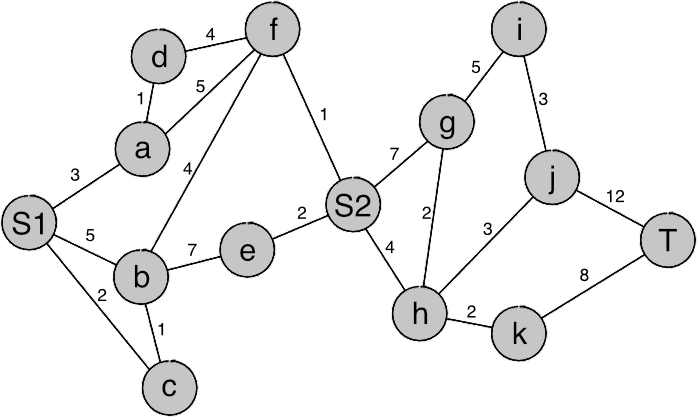
\includegraphics[scale=0.9]{chapters/informed_search/Anfangsproblem.png}
	\caption{Beispiel Graph}
\end{figure}

Wir sehen unsere Startknoten $S1$ und $S2$, sowie den Zielknoten $T$.  Au\ss erdem sind alle Kanten zwischen den Knoten mit einer L\"ange versehen. Im folgenden werden wir mit Hilfe der Breitensuche erst den Weg von $S1$ zu $T$ und dann den Weg von $S2$ zu $T$ suchen. In der folgenden Grafik sind die Zwischenknoten mit Kleinbuchstaben beschriftet, des weiteren sind Start und Ziel in gelb eingef\"arbt. In jedem Schritt werden die aktuell zu untersuchenden Knoten gr\"un und die bereits besuchten Knoten blau markiert.

\begin{figure}[h!]
	\centering
	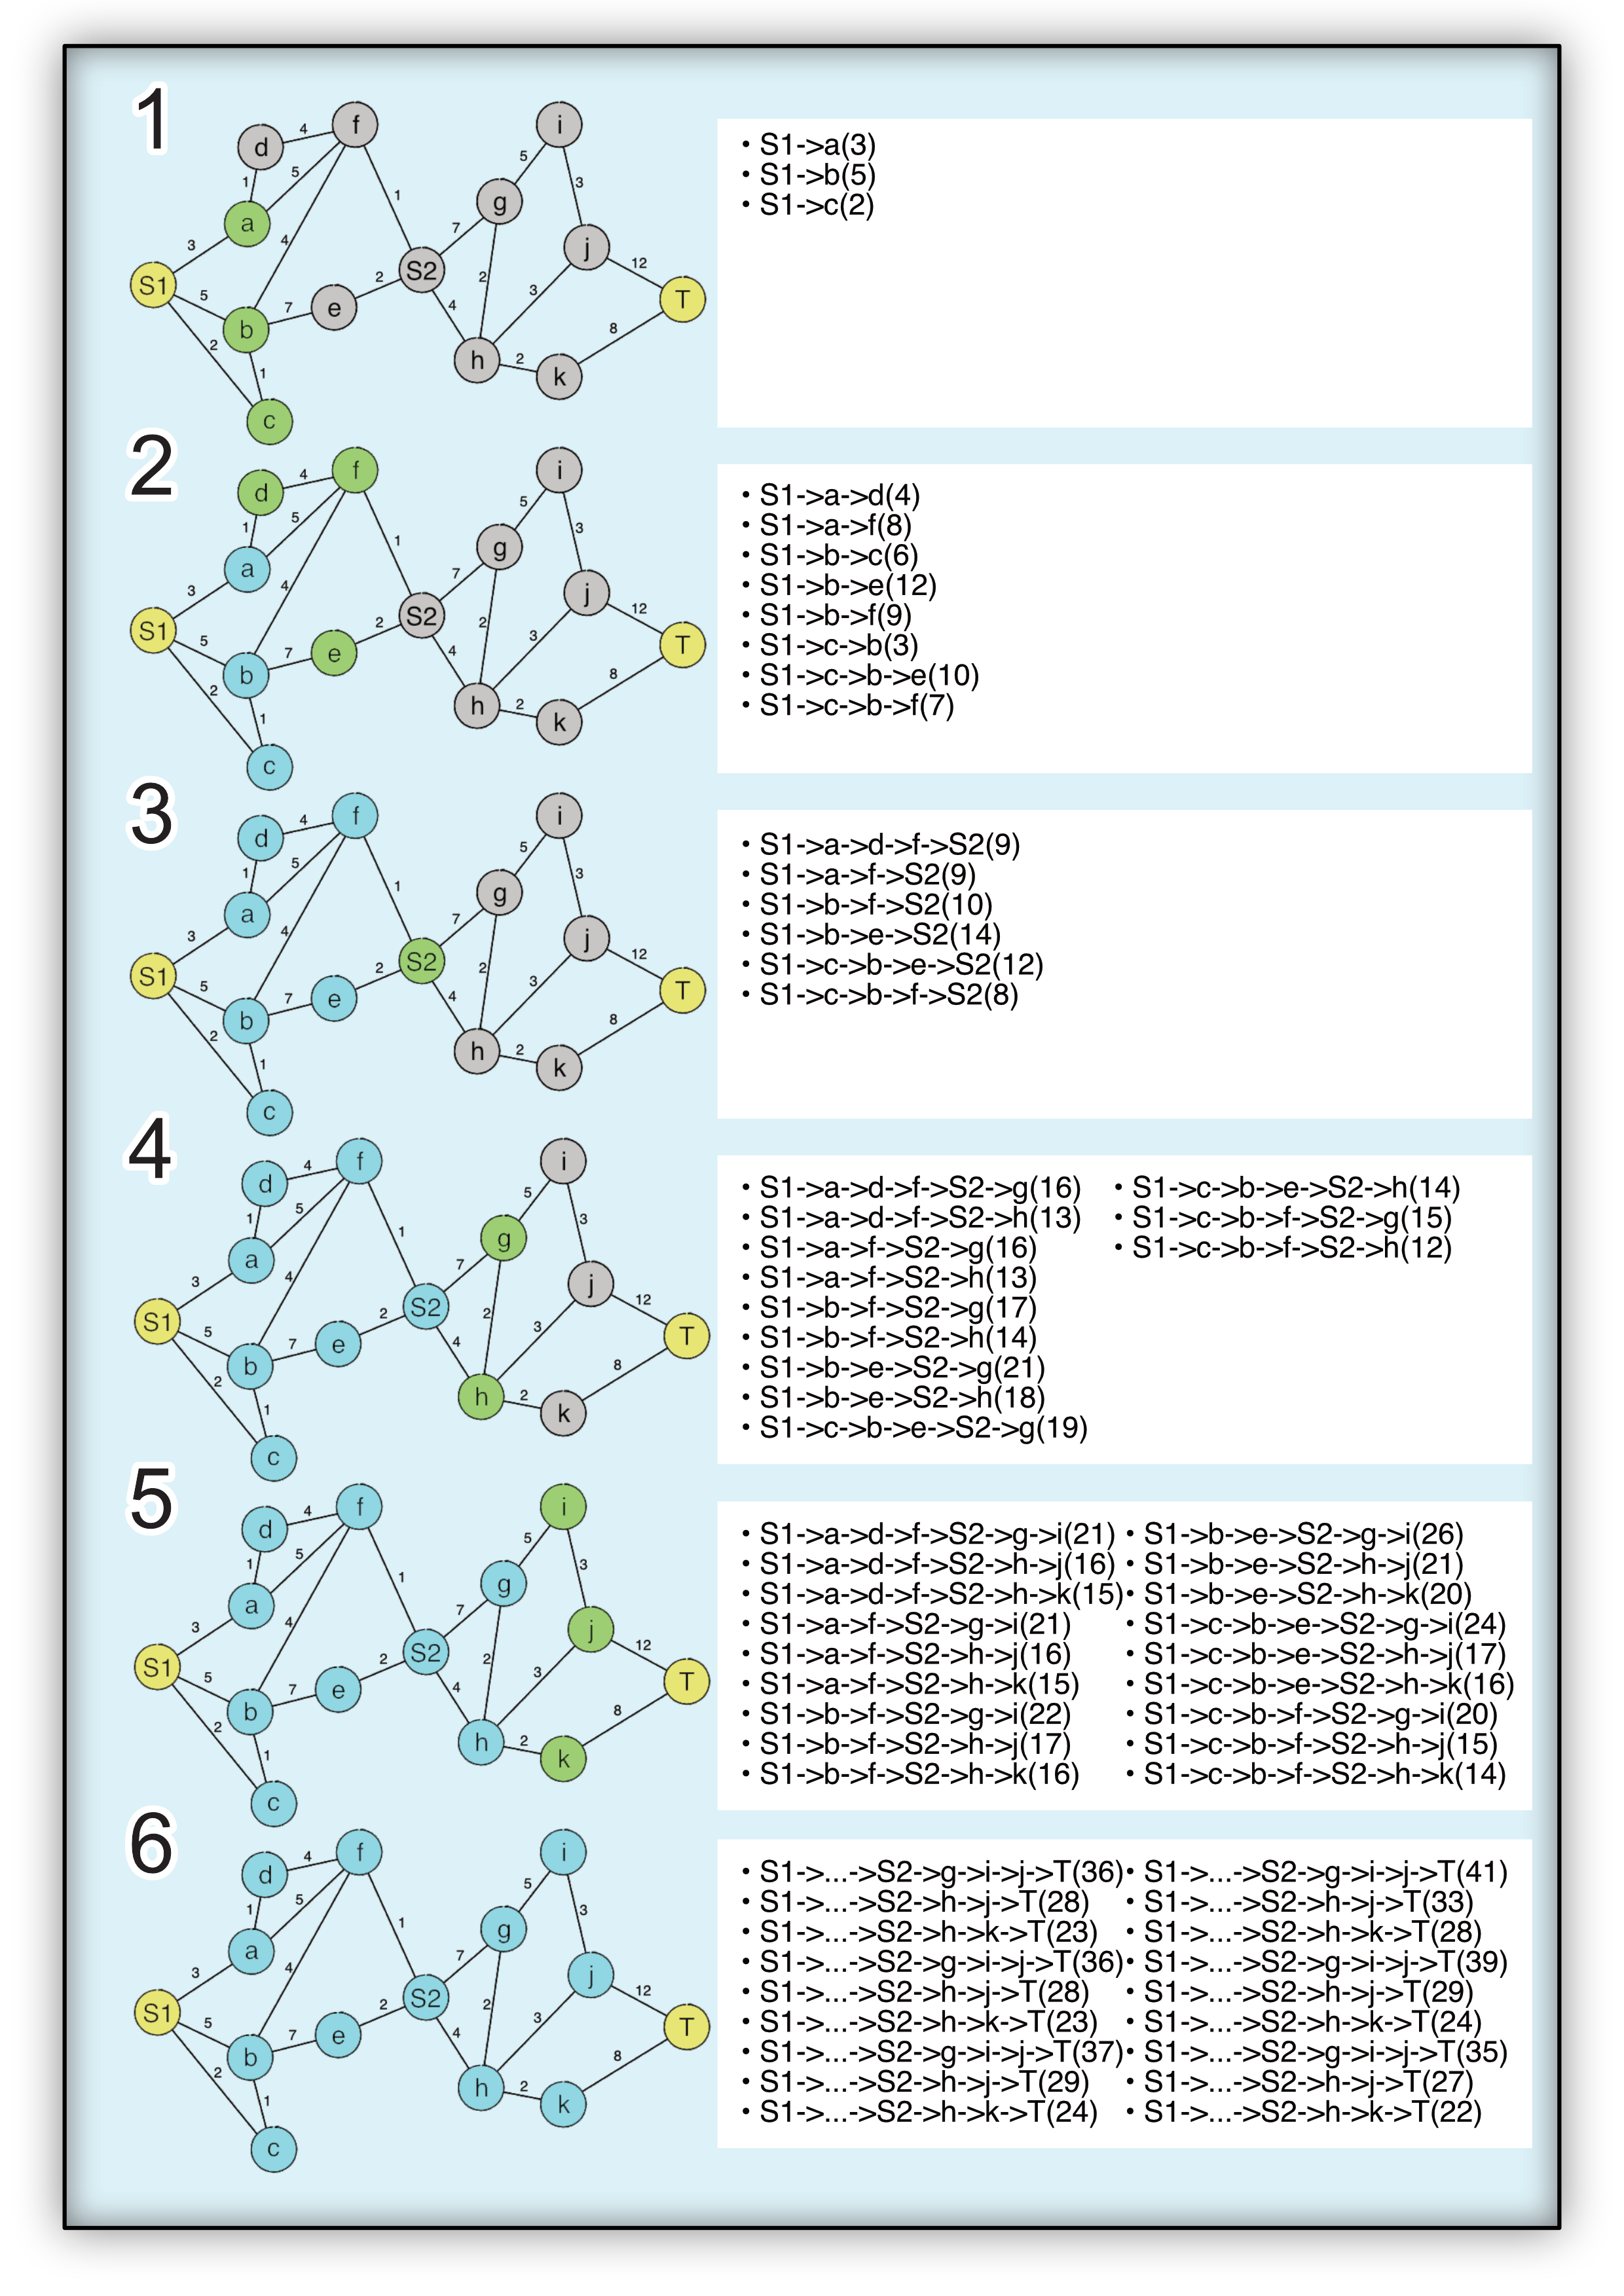
\includegraphics[scale=0.76]{chapters/informed_search/BeispielGraphen1.png}
	\caption{Beispiel Graph mit Breitensuche. Zu jedem Graphen sind die besuchten Wege angegeben. Die durch "..."\ zusammengefassten Wegst\"ucke der Wege des letzten Graphen entsprechen denen der Wegen von $S1$ nach $S2$ des vorletzten Graphens.}
\end{figure}

\begin{enumerate}
	\item Wir besuchen zuerst Knoten $a$, $b$ und $c$ und stellen offensichtlich fest, dass wir $T$ noch nicht erreicht haben. 
	\item Wir besuchen nun $d$, $e$ und $f$. Wir haben $T$ immer noch nicht erreicht.
	\item In diesem Schritt gibt es nur $S2$ zu besuchen. 
	\item Ab hier Suchen wir effektiv den k\"urzesten Weg von $S2$ zu $T$, weshalb dieses Beispiel sp\"ater nicht mehr extra erl\"autert wird. Hier besuchen wir die Knoten $g$ und $h$.
	\item Dann besuchen wir noch $i$, $j$ und $k$.
	\item Jetzt bilden wir noch die letzen Wege und diese enden beim Knoten $T$. Also sind wir fertig. 
\end{enumerate}
Der k\"urzeste Weg von $S1$ zu $T$ ist also:
\begin{itemize}
	\item  $S1\rightarrow c\rightarrow b\rightarrow f\rightarrow S2\rightarrow h\rightarrow k\rightarrow T$
\end{itemize}
Und daraus folgt der k\"urzeste Weg von S2 zu T ist: 
\begin{itemize}
	\item $S2\rightarrow h\rightarrow k\rightarrow T$
\end{itemize}
Fazit:

Wie man sieht ist das Problem gut l\"osbar mit uninformierte Suche, aber es f\"allt sofort auf das wir alle Knoten besuchen mussten und alle Wege bilden mussten.
Dies hat nicht nur hohe Speicherkosten zur Folge, sondern auch eine hohe Laufzeit. 
Bereits bei diesen simplen Beispiel sieht man die enorme Menge von Wegen die man speichern muss. 
Als Mensch w\"urde man bei dieser Suche weniger Wege betrachten:
\begin{itemize}
	\item W\"are es nicht einfacher Wege auszulassen die offensichtlich zu lang sind?
	\item Oder w\"are es nicht besser Wege wie $S1\rightarrow b$ durch den k\"urzeren $S1\rightarrow c\rightarrow b$ zu ersetzen?
\end{itemize}
Unterbewusst benutzt man eine Menge Vereinfachungen die der Computer vielleicht auch anwenden sollte. 
Im folgenden Kapitel werden wir versuchen diese Suche intuitiv zu optimieren. /newpage

\section{Verbesserungen}
\subsection{Intuitiver Algorithmus}
Statt alle Knoten zu besuchen wie bisher, werden wir im folgenden unser Wissen \"uber den Graphen nutzen um schneller zum Ergebnis zu kommen. Folgende Regeln werden angewandt:
\begin{enumerate}
	\item Wir besuchen immer den Knoten mit der niedrigsten Kantenl\"ange zuerst.
	\item Wenn wir einen neuen Weg zu einem Knoten finden und dieser k\"urzer ist als der vorherige, brauchen wir nur noch diesen neuen Weg zu betrachten. Ansonsten kann der neue Weg ignoriert werden.
	\item Wenn wir zwei Wege zur Auswahl haben, die gleichlang sind, w\"ahlen wir zuf\"allig.
	\item Wenn ein Weg keine nicht besuchten Kinder mehr hat gehen wir zur\"uck zum letzten Knoten der noch offene Kinder hatte.
	\item Aufgrund der oben genannten Regeln muss der erste Weg zum Ziel der k\"urzeste sein. (Um das Beispiel nicht unn\"otig lang zu machen, wird dies an dieser Stelle nicht bewiesen)
\end{enumerate}

\subsection{Anwendung}
Wir beginnen mit dem Graphen aus Kapitel 1. Die Knoten werden genau wie bereits bekannt eingef\"arbt werden. 

\begin{figure}[h!]
	\centering
	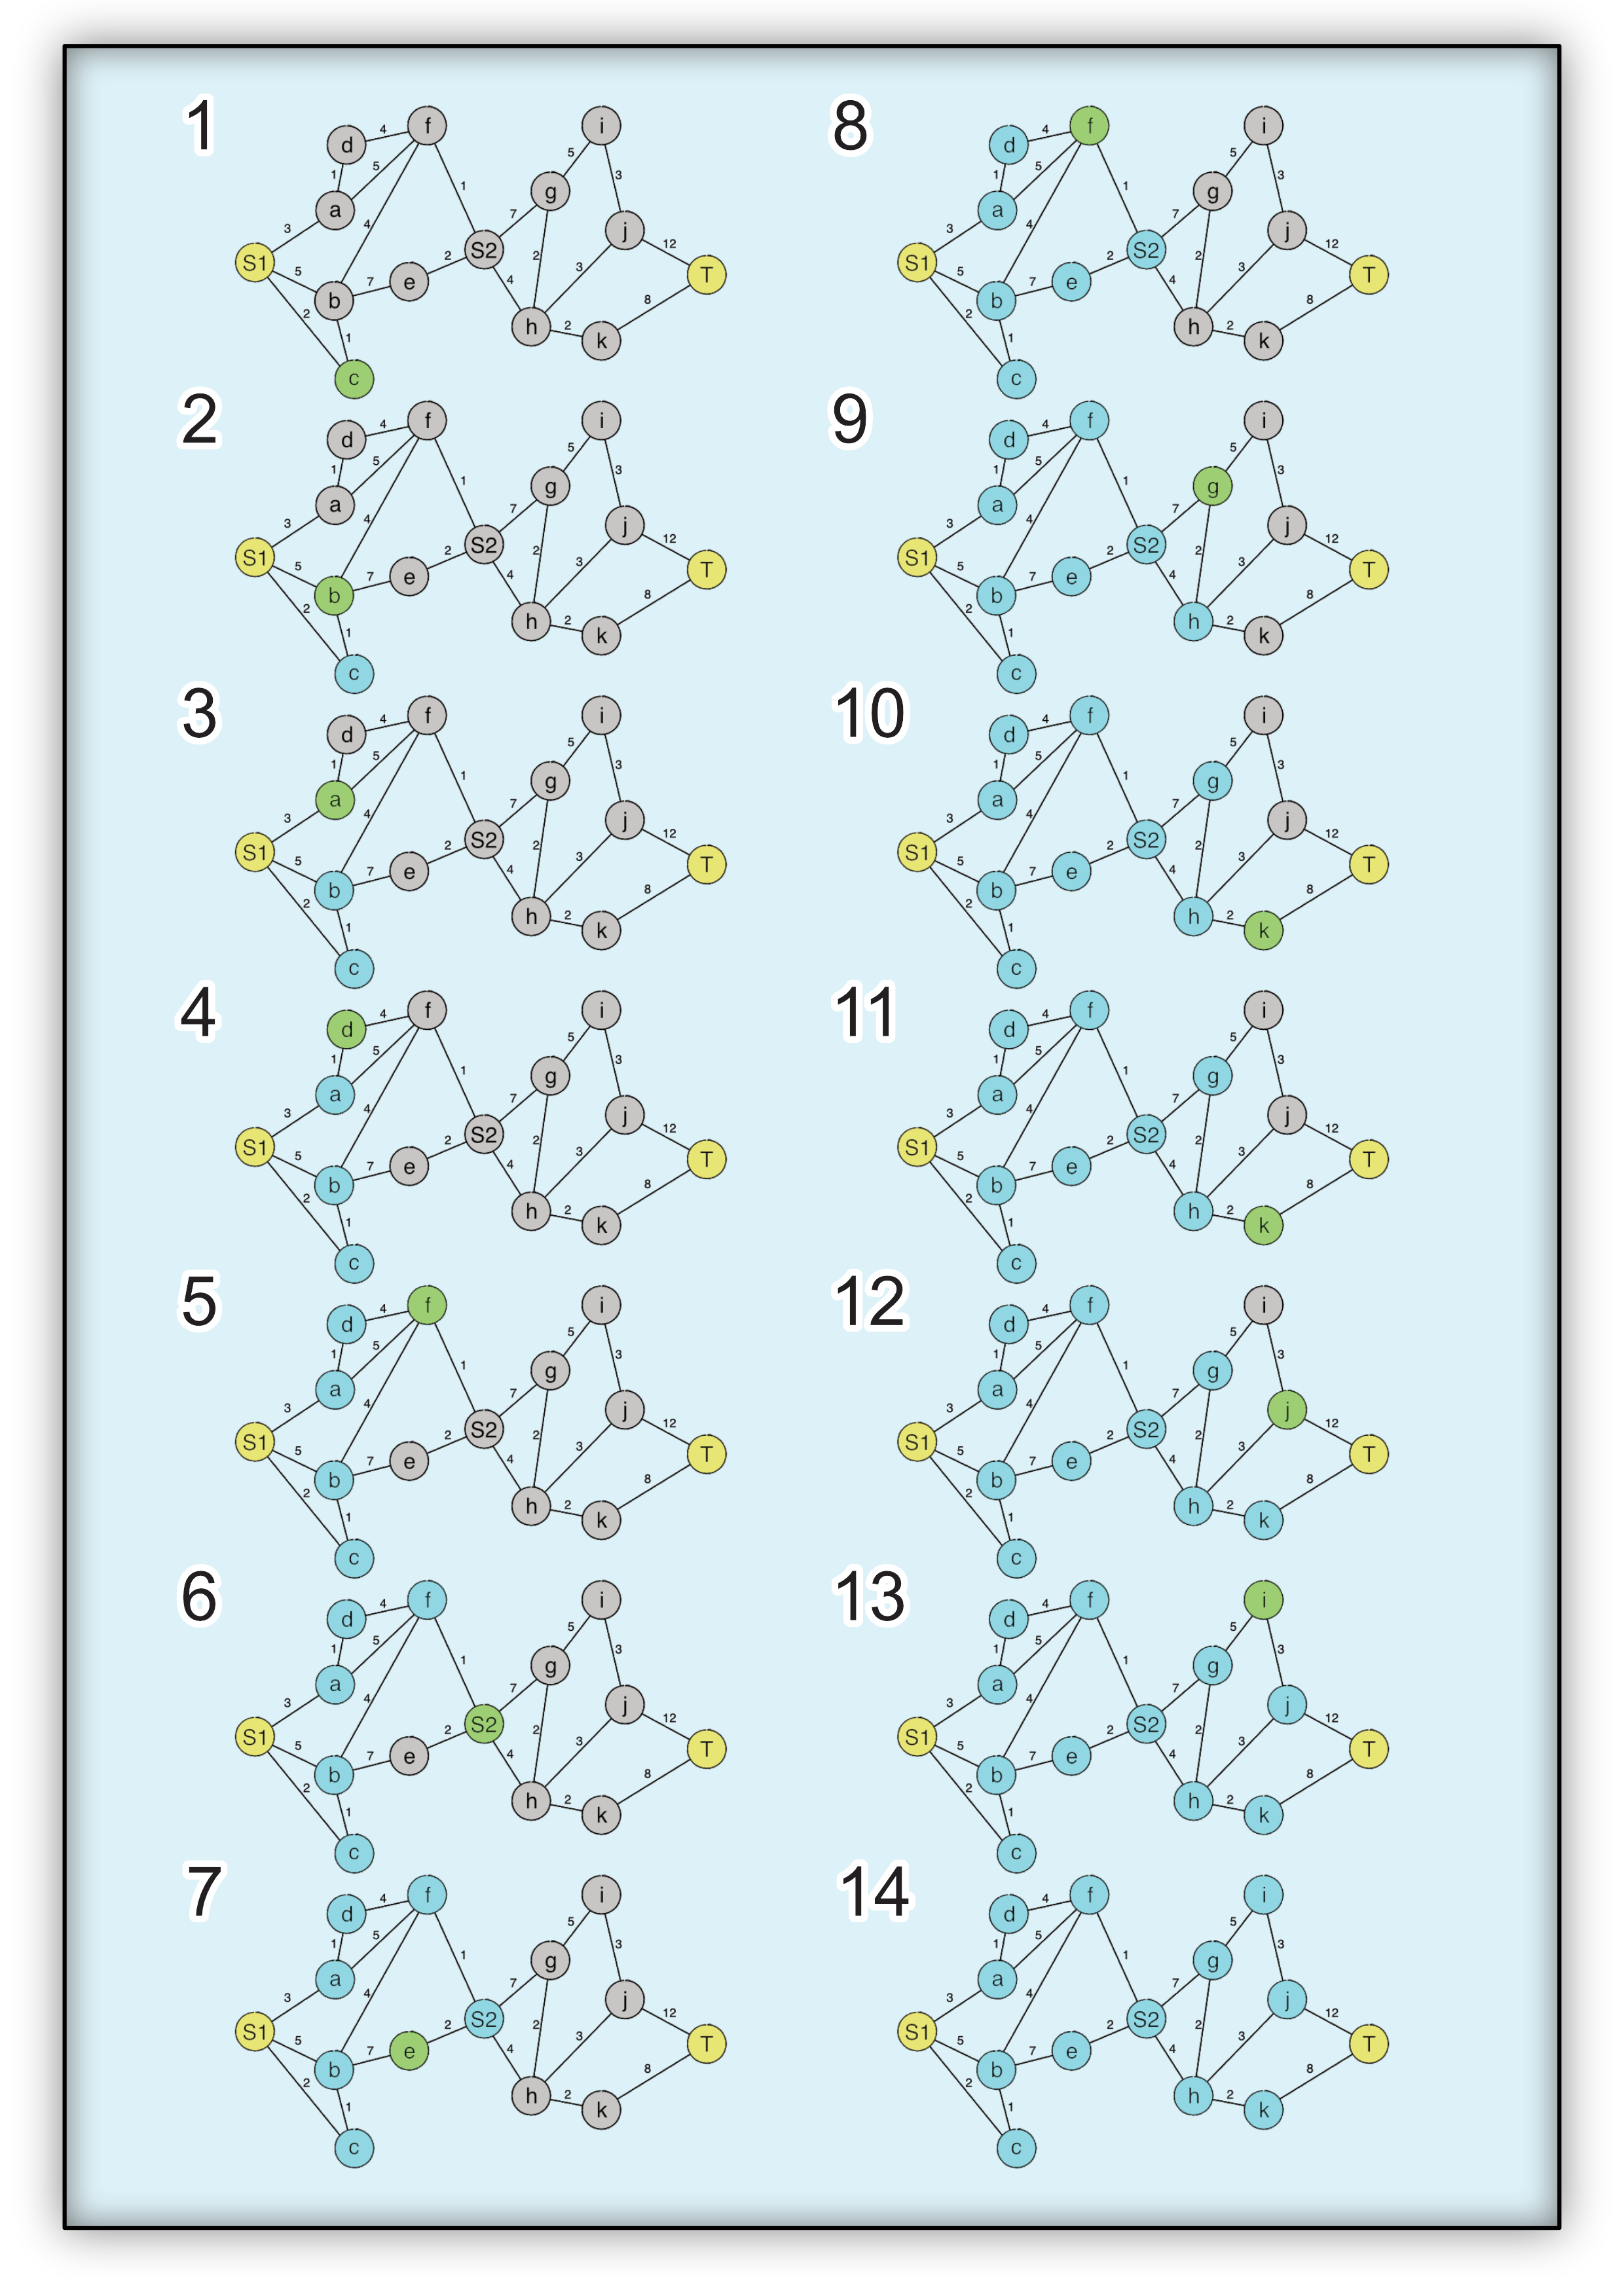
\includegraphics[scale=0.76]{chapters/informed_search/BeispielGraphen2.png}
	\caption{Beispiel Graph mit intuitiven Algorithmus.}
\end{figure}

\begin{enumerate}	\item Wir beginnen mit Knoten $c$ da mit einer L\"ange von $2$ seine Kante am k\"urzesten ist $(Regel 1)$. 
Wir haben also den Weg:
	\begin{itemize}
		\item $S1\rightarrow c(2)$
	\end {itemize}
	\item Nun besuchen wir $b$ und erhalten den Weg:
	\begin{itemize}
		\item $S1\rightarrow c\rightarrow b(3)$
	\end{itemize}
	\item Jetzt m\"ussen wir erst $a$ betrachten, da die Kante mit einer L\"ange von $3$ k\"urzer ist als $b\rightarrow f$ mit $4$. Wir haben also die Wege:
	\begin{itemize}
		\item $S1\rightarrow c\rightarrow b(3)$
		\item $S1\rightarrow a(3)$
	\end{itemize}
	\item Als n\"achstes besuchen wir $d$, da $a\rightarrow d$ am k\"urzesten ist. Es werden die Wege:
	\begin{itemize}
		\item $S1\rightarrow c\rightarrow b(3)$
		\item $S1\rightarrow a\rightarrow d(4)$
	\end{itemize}
	gespeichert.	\item Wir mussten uns zwischen $d\rightarrow f$ und $b\rightarrow f$ entscheiden und haben zuf\"allig $d\rightarrow f$ gew\"ahlt $(Regel 3)$. Damit ergeben sich die Wege:
	\begin{itemize}
		\item $S1\rightarrow c\rightarrow b(3)$
		\item $S1\rightarrow a\rightarrow d\rightarrow f(8)$
	\end{itemize}
	\item Im n\"achsten Schritt w\"ahlen wir $f\rightarrow S2$. Die Wege sind:
	\begin{itemize}
		\item $S1\rightarrow c\rightarrow b(3)$
		\item $S1\rightarrow a\rightarrow d\rightarrow f\rightarrow S2(9)$
	\end{itemize}
	\item Jetzt besuchen wir $e$. Wir haben also die Wege:
	\begin{itemize}
		\item $S1\rightarrow c\rightarrow b(3)$
		\item $S1\rightarrow a\rightarrow d\rightarrow f\rightarrow S2\rightarrow e(11)$
	\end{itemize}
	Stellen aber fest, dass $e$ f\"ur den n\"achsten Schritt keine unbesuchten Kinder hat. Also gehen wir zur\"uck zu $S2$ da dieser noch Kinder hatte $(Regel 4)$. Die Wege werden wieder zu:
	\begin{itemize}
		\item $S1\rightarrow c\rightarrow b(3)$
		\item $S1\rightarrow a\rightarrow d\rightarrow f\rightarrow S2(9)$
	\end{itemize}
	Wir besuchen noch einmal $f$, dieses Mal als $b\rightarrow f$ (zuf\"allig gew\"ahlt aus $b\rightarrow f$ und $S2\rightarrow h$). Damit haben wir einen neuen Weg zu $f$, der k\"urzer ist als $S1\rightarrow a\rightarrow d\rightarrow f$. Wir ersetzen ihn $(Regel 2)$. Damit ergibt sich der Weg:
	\begin{itemize}
		\item $S1\rightarrow c\rightarrow b\rightarrow f\rightarrow S2(8)$
	\end{itemize}	\item Wir w\"ahlen $h$ und erhalten den Weg:
	\begin{itemize}
		\item $S1\rightarrow c\rightarrow b\rightarrow f\rightarrow S2\rightarrow h(12)$
	\end{itemize}
	\item Aus $h\rightarrow g$ und $h\rightarrow k$ w\"ahlen wir $g$. Der Weg ist:
	\begin{itemize}
		\item $S1\rightarrow c\rightarrow b\rightarrow f\rightarrow S2\rightarrow h\rightarrow g(14)$
	\end{itemize}
	\item Wir besuchen $k$. Damit ergeben sich die Wege:
	\begin{itemize}
		\item $S1\rightarrow c\rightarrow b\rightarrow f\rightarrow S2\rightarrow h\rightarrow g(14)$
		\item $S1\rightarrow c\rightarrow b\rightarrow f\rightarrow S2\rightarrow h\rightarrow k(14)$
	\end{itemize}
	\item Wir w\"ahlen $j$ und erhalten die Wege: 
	\begin{itemize}
		\item $S1\rightarrow c\rightarrow b\rightarrow f\rightarrow S2\rightarrow h\rightarrow g(14)$
		\item $S1\rightarrow c\rightarrow b\rightarrow f\rightarrow S2\rightarrow h\rightarrow k(14)$
		\item $S1\rightarrow c\rightarrow b\rightarrow f\rightarrow S2\rightarrow h\rightarrow j(15)$
	\end{itemize}	\item Jetzt besuchen wir erst $j\rightarrow i$. 
	\item Dann besuchen wir sofort $g\rightarrow i$, aber wir haben \"uber $j$ bereits einen k\"urzeren Weg zu $i$ und k\"onnen den neuen ignorieren. Es folgen die Wege:
	\begin{itemize}
		\item $S1\rightarrow c\rightarrow b\rightarrow f\rightarrow S2\rightarrow h\rightarrow k(14)$
		\item $S1\rightarrow c\rightarrow b\rightarrow f\rightarrow S2\rightarrow h\rightarrow j\rightarrow i(18)$
	\end{itemize}
	Und wir sehen, dass $i$ keine Kinder mehr hat:
	\begin{itemize}
		\item $S1\rightarrow c\rightarrow b\rightarrow f\rightarrow S2\rightarrow h\rightarrow k(14)$
		\item $S1\rightarrow c\rightarrow b\rightarrow f\rightarrow S2\rightarrow h\rightarrow j(15)$
	\end{itemize}
	\item Als letztes nehmen wir noch $k \rightarrow  T$. Wir bekommen also den Weg:
	\begin{itemize}
		\item $S1 \rightarrow  c \rightarrow  b \rightarrow  f \rightarrow  S2 \rightarrow  h \rightarrow  k \rightarrow  T (22)$ 
	\end{itemize}
	und aus $Regel 5$ folgt, dass dies der k\"urzeste Weg sein muss. 
\end{enumerate}
Fazit:

Zuallererst unser Ergebnis ist identisch mit dem aus Kapitel 1, wir haben also ebenfalls den besten Weg gefunden.  Es es leicht sichtbar, dass unser intuitiver Algorithmus nicht perfekt ist. Wir mussten trotzdem alle Knoten besuchen, genau wie die Breitensuche. Aber man sieht ebenfalls sofort, dass wir deutlich weniger Wege betrachten und speichern mussten als zuvor. Und besonders hervorzuheben ist, dass wir die Suche beenden konnten als wir den ersten Weg gefunden hatten. Das wirkt sich nat\"urlich positiv auf Laufzeit und Speicherverbrauch aus. In den folgenden Kapiteln wollen wir die hier intuitiv erarbeiteten Konzepte formal definieren, die echten Algorithmen der informierten Suche vorstellen und deren Eigenschaften \"uberpr\"ufen. 
 
\section{Einleitung}
Statt blind alle M\"oglichkeiten zu probieren um die Beste zu erhalten, zieht man, wie ein Mensch es intuitiv machen w\"urde, weitere Informationen \"uber das Problem zurate (Heuristiken) und ignoriert L\"osungen die offensichtlich schlechter sind als bereits gefundene (Branch and Bound). Damit ergibt sich eine deutlich bessere Laufzeit, wie sie in Echtzeitanwendungen (z.B. in Spielen) n\"otig ist. Nat\"urlich stellt sich auch die Frage, ob diese einfacher erhaltene L\"osung immer noch die optimale L\"osung ist (Optimalit\"at). Im folgenden werden die Verschiedenen Arten (Best-First Search und A*) informierter Suche von und deren Vor- und Nachteile erkl\"art. 

\section{Definitionen}
\subsection{Branch and Bound}
Branch and Bound (h\"aufig abgek\"urzt mit B\&B\footnote{Branch and Bound Algorithms - Principles and Examples. Jens Clausen, March 12, 1999}) ist eine Optimierungsstrategie f\"ur Algorithmen, hier im speziellen Suchverfahren. Um nicht alle Knoten eines Baumes durchsuchen zu m\"ussen, kann man, wie bereits intuitiv oben gesehen, die Aufgabe in Teile aufteilen ("Branch"\ engl. "to branch" verzweigen\footnote{www.dict.cc}) und diese Teile nach Relevanz f\"ur die L\"osung einteilen ("Bound\ engl. "to bound" beschr\"anken\footnote{www.dict.cc}). 
Damit man dies bei Suchalgorithmen bewerkstelligen kann benutzt man eine Absch\"atzung, intuitiv war dies "k\"urzeste Luftlinie zum Ziel"\, auch Heuristik genannt.\footnote{Anwendungen von Branch and Bound, Frederik Wollny und Philipp Schmid, Hochschule Aalen, 2016}

\subsection{Extended List}
Bei der Anwendung von Branch and Bound kann es dazu kommen, dass Wege p'=(\dots, A) zu einen Knoten A weiter verfolgt werden, f\"ur die es einen Weg p=(\dots, A) gibt, so dass gilt:
\begin{center} 
$Wf(p) < Wf(p')$
\end{center}
Dies f\"uhrt dazu, dass der Suchbaum unn\"otig gro\ss wird. Um zu erreichen, dass nicht die l\"angeren Wege weiter verfolgt werden, wird die Extended List eingef\"uhrt. In der Extended List wird f\"ur jeden Knoten zum Zeitpunkt an dem dieser besucht wird, die Knoten Identifikation und die Wegl\"ange zu diesem gespeichert. F\"uhrt nun im Verlauf der Suche ein Weg zu einem Knoten, der bereits in der Extended List gespeichert ist, so wird die gespeicherte mit der Aktuellen Wegl\"ange zum Knoten verglichen. Ist die Aktuelle Wegl\"ange gr\"o\ss er, muss der Weg nicht weiter verfolgt werden, es gibt bereits einen k\"urzeren Weg zu dem Knoten. Ist sie geringer, wird der neue Wert eingetragen und der \"altere Weg \"uber diesen Knoten muss nicht weiter betrachtet werden.\footnote{https://ocw.mit.edu/courses/electrical-engineering-and-computer-science/6-034-artificial-intelligence-fall-2010/lecture-videos/lecture-5-search-optimal-branch-and-bound-a/} Mit Branch and Bound + Extended List ergibt sich in unserem Beispiel Graphen:

\begin{figure}[h!]
	\centering
	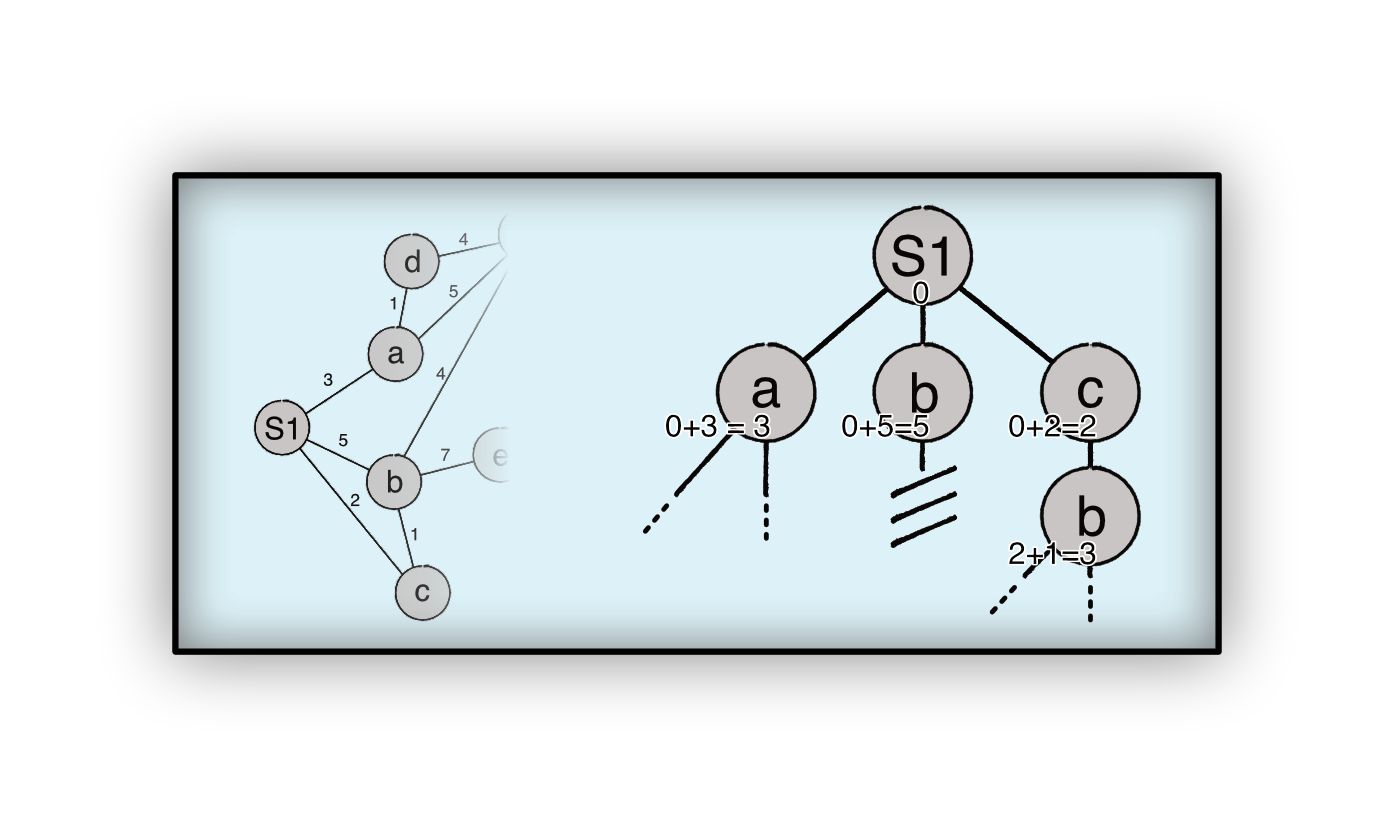
\includegraphics[scale=0.4]{chapters/informed_search/ExtendedListBeispiel.png}
	\caption{Links ist der linke Teil des Beispiel Graphen abgebildet, rechts ein Teil des Suchbaums von Branch and Bound + Extended List. Wie abgebildet wird der Weg (S1, b, \dots) nicht weiter verfolgt, da, $Wf((S1, c, b)) < Wf(S1,b)$.}
\end{figure}

\section{Best-First Search}
Best-First Search ist eine Klasse von informierten Such-Algorithmen, welche nachdem Prinzip arbeiten, dass sie stets denjenigen Knoten zuerst untersuchen, welcher f\"ur den Erfolg der Suche am "vielversprechendsten"\ erscheint. Die Wahl dieses "vielversprechenden"\ Knotens geschieht anhand einer gewissen Heuristik. Der wohl bekannteste Algorithmus aus diesem Bereich ist A*, welcher auch als eine Erweiterung von Branch and Bound gesehen werden kann. An ihm wollen wir im Folgenden das Prinzip von Best-First Search verdeutlichen. 

\section{Heuristik}
Die Heuristik ist im Falle der Informierten Suche die Representation der menschlichen L\"osungsfindung im Such-Algorithmus. Sie weist jedem Knoten einen gesch\"atzten Wert zu, der dar\"uber Auskunft gibt, ob es sich lohnen k\"onnte, einen Weg \"uber diesen Knoten einzuschlagen. Bei der Findung des k\"urzesten Weges gilt, desto h\"oher der durch die Heuristik bestimmte Wert f\"ur einen Knoten ist, desto unwahrscheinlicher ist es, dass der K\"urzeste Weg \"uber diesen Knoten verl\"auft. Aufgrund der Vielfalt von Gegebenheiten unter denen eine Suche stattfinden kann, ist es offensichtlich, dass eine Heuristik die ein Problem L\"ost nicht ohne weiteres auf andere Probleme \"ubertragen werden kann. Deswegen werden zun\"achst einige wichtige Begrifflichkeiten gekl\"art, die beim Umgang mit Heuristiken helfen k\"onnen.\footnote{http://www.duden.de/rechtschreibung/Heuristik}

\subsection{Eigenschaften von Heuristiken}
Im folgenden werden einige Eigenschaften definiert, die eine Heuristikfunktion erf\"ullen kann. Diese Eigenschaften k\"onnen dabei helfen ein Urteil, \"uber die Zul\"assigkeit einer Heuristik f\"ur eine Problemstellung, zu f\"allen.
\newtheorem*{theore}{Theorem}
\theoremstyle{definition}
\newtheorem*{defi}{Definition}

\begin{defi}
Eine heuristische Funktion $h(n)$ wird als admissible (zul\"assig) bezeichnet, wenn f\"ur alle Knoten $n$ erf\"ullt ist: 
\begin{center}
$h(m) \leq k(m, n)$
\end{center}
mit $k(m, n)$ als k\"urzeste Wegl\"ange von $m$ nach $n$ und f\"ur alle Knoten $t \in G$, die die Endbedingung erf\"ullen, gilt: 
\begin{center}
$h(t)=0.\footnote{https://ocw.mit.edu/courses/electrical-engineering-and-computer-science/6-034-artificial-intelligence-fall-2010/lecture-videos/lecture-5-search-optimal-branch-and-bound-a/}$
\end{center}
\end{defi}

Admissible Heuristiken reichen bereits aus, um auf Landkarten o.\"a. nach der k\"urzesten Route zu suchen. Damit eine Heuristik auch f\"ur Suchen verwendet werden kann die nicht auf geografischer Ebene stattfinden, werden die Eigenschaften konsistent und monoton definiert. Die Definitionen wurden aus [Kai13] \"ubernommen. 

\begin{defi}
Eine heuristische Funktion $h(n)$ ist konsistent, wenn f\"ur alle Knotenpaare $m, n \in G$ folgendes erf\"ullt ist: 
\begin{center}
$h(m) \leq k(m, n) + h(n)$
\end{center}
mit $k(m, n)$ als k\"urzeste Wegl\"ange von $m$ nach $n$ und f\"ur alle Knoten $t \in G$, die die Endbedingung erf\"ullen, gilt: 
\begin{center}
$h(t)=0$.
\end{center}
\end{defi}

\begin{defi}
Eine heuristische Funktion $h(n)$ ist monoton, wenn f\"ur alle Knotenpaare $m, n \in G$ mit $n$ als unmittelbarem Nachbar von $m$ folgendes erf\"ullt ist: 
\begin{center}
$h(m) \leq c(m, n) + h(n)$
\end{center}
mit $c(m, n)$ als Kosten der Kante von $m$ nach $n$; und f\"ur alle Knoten $t \in G$, die die Endbedingung erf\"ullen, gilt: 
\begin{center}
$h(t)=0$.
\end{center}
\end{defi}

\begin{theore}
Die Eigenschaften konsistent und monoton sind \"aquivalent.
\end{theore}

\begin{theore}
F\"ur jede konsistente Funktion $h$ gilt:
$h(n) \leq h*(n)$ f\"ur alle Knoten $n \in G$.
\end{theore}

Um den unterschied zwischen einer Heuristik die admissible ist und einer die konsistent ist zu verdeutlichen, sei ein Beispiel angef\"uhrt: 

\begin{figure}[h!]
	\centering
	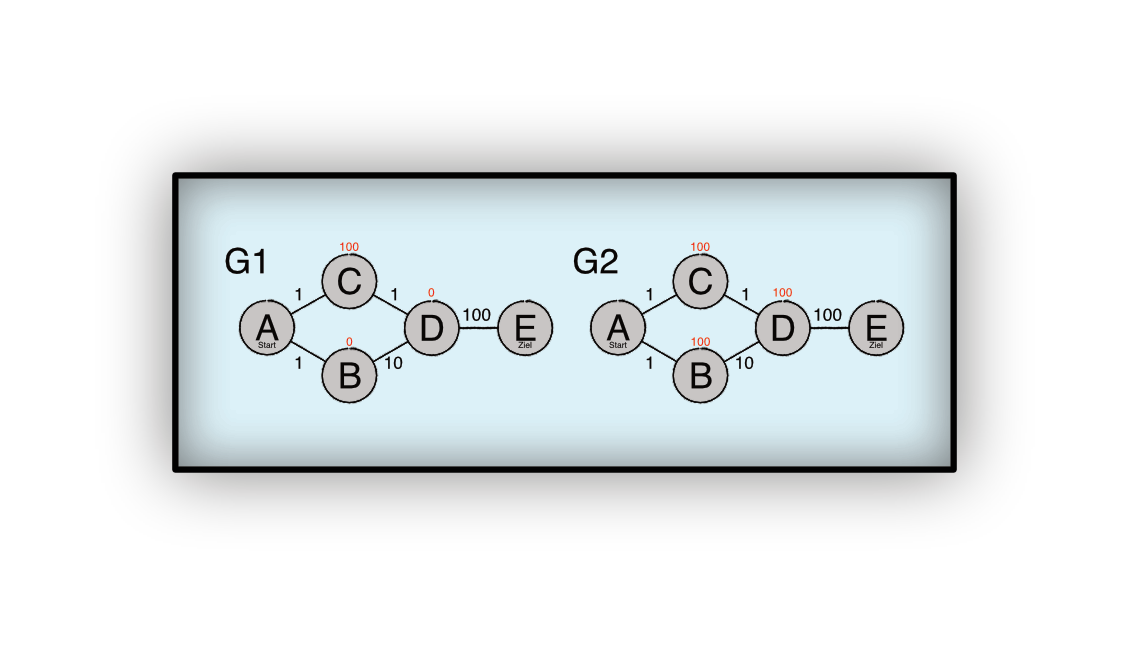
\includegraphics[scale=0.5]{chapters/informed_search/BeispielHeuristik.png}
	\caption{Die Abbildungen G1 und G2 beschreiben das selbe Problem mit zwei verschiedenen Heuristiken. Ziel ist es den k\"urzesten Weg von Knoten A nach Knoten E zu finden. G1 stellt die Verwendung einer admissible Heuristik und G2 die einer konsistenten Heuristik dar. Die roten Zahlen geben die Werte der Heuristikfunktionen an den relevanten Knoten an. Wird nun eine Suche, mit Branch and Bound + Extended List + Heuristik durchgef\"uhrt, liefert die Suche f\"ur G1 den Weg(A,B,D,E) und f\"ur G2 den Weg(A,C,D,E). Entscheidend f\"ur diese L\"osung ist, dass bei G1 zun\"achst A,B, und D betrachtet werden und somit aufgrund der Extended List der Weg (A,C,D,E) wegf\"allt. Im Gegensatz dazu beginnt die Suche bei G2 mit einem Weg \"uber C, da die gesch\"atzten Kosten von C mit 101 kleiner als die von B sind.}
\end{figure}

\subsection{Verschiedene Heuristiken}
In diesem Abschnitt werden drei Heuristiken vorgestellt, angefangen mit der Hamming-Distanz. Aufgrund dessen, dass in einigen Kapiteln Bezug auf die folgenden Heuristiken genommen wird, wurden einige Bezeichnungen in den Definitionen entsprechend angepasst.\\
Die Hamming-Distanz hh(m,n) beschreibt wie gro\ss der Unterschied zwischen den Zeichenketten m und n ist und ist wie folgt definiert: 
\begin{defi}
$\sum$ sei ein endliches Alphabet sowie $m = (m_{1}, \dots, m_{k})$ und $y = (n_{1}, \dots, n_{k})$ zwei $k$ Zeichen lange Worte aus $\sum^{k}$. Die Hamming-Distanz zwischen $m$ und $n$ ist definiert als:
\begin{center}
$h_{h}(m,n) := |{j \in \{1 , \dots , k\} | m_{j} \neq n_{j}}|$.
\end{center}
\end{defi}
Eine Heuristik w\"are z.B. $h(n)=h_{h}(n,x)$, mit $x$ als Ziel-Konstellation der Suche.\footnote{http://sb.fluomedia.org/hamming/, https://de.wikipedia.org/wiki/Hamming-Abstand}
\begin{defi}
Die Manhattan Distanz $h_{m}(m,n)$ f\"ur die Punkte $n$ und $m$ beschreibt die Distanz, die zustande kommt, wenn nur horizontale und vertikale Wege genommen werden, um $n$ von $m$ aus zu erreichen. Die Manhattan-Distanz ist wie folgt definiert:
\begin{center}
$h_{m}(m,n) = \sum_{i} |m_{i} - n_{i}|.$
\end{center}
\end{defi}
Eine Heuristik w\"are z.B $h(n)=h_{m}(n,x)$, mit $x$ als Ziel-Knoten der Suche.\footnote{http://mathworld.wolfram.com/TaxicabMetric.html}
\begin{defi}
Der Euklidischer Abstand $h_{e}(m,n)$ von $m$ und $n$ entspricht der "Luftlinie" zwischen diesen. Der Euklidische Abstand f\"ur zwei Vektoren im $k$-Dimensionalen Raum ist wie folgt definiert:
\begin{center}
$h_{e}(m,n) =\sqrt{((m_{1} - n_{1})^{2}+\dots+(m_{k} - n_{k})^{2})}.$
\end{center}
\end{defi}
Eine Heuristik w\"are z.B $h(n)= h_{e}(n,x)$, mit $x$ als Ziel-Knoten der Suche.\footnote{http://mathworld.wolfram.com/EuclideanMetric.html}

\subsection{Findung von Bewertungsfunktionen}
Die Frage Lautet:"Wie findet sich die richtige Heuristikfunktion f\"ur die gegebene Problemstellung". Um einen L\"osungsansatz f\"ur eine allgemeine Vorgehensweise zu finden, wird zun\"achst das Beispiel aus 5.1 betrachtet. Die Aufgabe im Beispiel ist es, den k\"urzesten Weg von dem Knoten S1 bzw. S2 zum Zielknoten T im Graphen zu finden. Die Problemstellung l\"asst sich in eine Konjunktion von zwei Bedingungen aufteilen:
\begin{enumerate}
	\item Die zur\"uckgelegte Strecke von S1 bzw. S2 nach T soll minimal sein.
	\item Die Strecke entspricht einem Weg (Graphentheorie).
\end{enumerate}
W\"urde die zweite Bedingung weggelassen, w\"urde immer eine Strecke entsprechend der Luftlinie von $S1$ bzw. $S2$ nach $T$ gew\"ahlt werden. Es liegt also nahe $h(n)=h_{e}(n,x)$ zu w\"ahlen, um einem Knoten nach seiner Distanz zu $T$ zu bewerten. Wird Bedingung zwei nun hinzugezogen, werden mit der gew\"ahlten Heuristik immer die erreichbaren Knoten bevorzugt, die am n\"achsten zum Ziel liegen. So ist eine Akzeptable Heuristik f\"ur die Problemstellung gefunden. Dieses Prinzip des Konstruieren von vereinfachten Modellen durch systematisches Weglassen von Bedingungen der Konjunktion der Problemstellung scheint auch allgemein eine gute Herangehensweise zu sein, um leicht heuristische Sch\"atzungen zu ermitteln.

\section{A* Algorithmus}
A* beschreibt eine Gruppe von Algorithmen, die auf alle Kniffe der Informierten Suche, die bis jetzt vorgestellt wurden, zur\"uckgreifen:\footnote{https://ocw.mit.edu/courses/electrical-engineering-and-computer-science/6-034-artificial-intelligence-fall-2010/lecture-videos/lecture-5-search-optimal-branch-and-bound-a/}
\begin{itemize}
	\item Branch and Bound
	\item Extended List
	\item Heuristik
\end{itemize}
F\"ur ein gegebenes Problem gibt es innerhalb dieser Gruppe bessere und schlechtere Algorithmen. Um zwei A* Algorithmen zu vergleichen hilft das folgende Theorem: 

\begin{theore}
A*1 und A*2 seien zwei Versionen von A* mit $h1(n) ? h*(n)$ und $h2(n) ? h*(n)$ f\"ur alle Knoten $n \in G$ und mit $h1(n) ? h2(n)$ f\"ur alle Knoten $n \in G \ {t | t erf\"ullt die Endbedingung }$. (A*2 sei "besser informiert" als A*1.) Falls es eine L\"osung gibt, so wird bis zur Terminierung jeder von A*2 expandierte Knoten auch von A*1 expandiert, (A*2 "dominiert" A*1.)\footnote{[Kai13]} 
\end{theore}

In den folgenden Abschnitten wird auf weitere Eigenschaften des A* eingegangen und anschlie\ss end wird der A* durch Beispiele veranschaulicht. 

\subsection{Zul\"assigkeit}
Welche Bedingungen muss eine Heuristik erf\"ullen, damit unser Such-Verfahren ordnungsgem\"a\ss funktioniert? Dazu sollten wir zuerst definieren, wie wir uns ein korrekte Funktionsweise vorstellen.
\begin{itemize}
	\item Zul\"assigkeit Ein Such-Verfahren hei\ss t zul\"assig, falls es stets mit einer optimalen L\"osung terminiert, falls diese existiert.
\end{itemize}
Da bei unserem heuristischen Such-Verfahren A* die Wahl der Heuristik bisher nicht klar eingeschr\"ankt ist, liegt es nahe, dass in dieser Wahl ein entscheidender Punkt f\"ur die Zul\"assigkeit unseres Algorithmus liegt. Man kann sich leicht Heuristiken \"uberlegen, welche die Funktionsweise von A* st\"oren und daf\"ur sorgen, dass der Algorithmus keine optimale L\"osung findet oder wom\"oglich gar nicht erst terminiert. Wir sollten uns also genauer mit der Beschaffenheit von Heuristikfunktionen auseinandersetzen. Eine erste wichtige Eigenschaft einer Heuristik h zur Sch\"atzung von h* ist, ob diese optimistisch sch\"atzt.
\begin{itemize}
	\item optimistische Sch\"atzung Eine Sch\"atzung h von h* ist genau dann eine optimistische Sch\"atzung, falls sie die Kosten eines optimalen Pfades nie \"ubersch\"atzt.
\end{itemize}
Das heisst:
\begin{itemize}
	\item $h(n) \leq h*(n)$ f\"ur alle Knoten $n \in GP$
\end{itemize}

Diese Eigenschaft liefert uns nun die ausschlaggebende Bedingung f\"ur die Zul\"assigkeit von A*. Zul\"assigkeit von A*. Falls die verwendete Heuristik h eine optimistische Sch\"atzung von h* ist, dann ist A* zul\"assig. 
Der Beweis dieses Satzes und einige genauere Er\"orterungen k\"onnen in [Kai13] nachgelesen werden. 

\subsection{Komplexit\"at}
Es l\"asst sich leicht erkennen, dass A* in der Regel eine weit bessere Komplexit\"at hat, als blinde Such-Verfahren. Die Anzahl der expandierten Knoten ist bei A* oft sogar um ein Vielfaches geringer. Sei nun die L\"ange einer optimalen L\"osung mit d bezeichnet. Des Weiteren kann man von Einheitskosten ausgehen und die Existenz genau einer optimalen L\"osung voraussetzen. Je nachdem wie optimistisch nun der Fehler von h bez\"uglich h* angenommen wird, kommt man auf eine quadratische oder sogar lineare Komplexit\"at bez\"uglich d. Im eher realistischen Fall l\"asst sich jedoch nur auf eine exponentielle Komplexit\"at schliessen. 

\subsection{Optimalit\"at}
Nun interessieren wir uns f\"ur die Optimalit\"at von A* im Hinblick auf die Anzahl der expandierten Knoten. Der Begriff Optimalit\"at beruht hier auf dem der Dominanz. Das bedeutet, ein Verfahren ist optimal gegen\"uber einer Klasse von Verfahren, wenn es alle Elemente aus dieser Klasse dominiert. F\"ur den ganz allgemeinen Fall l\"asst sich leicht erkennen, dass A* nicht das optimale Verfahren \"uberhaupt ist. Es gibt in bestimmten F\"allen offensichtlich Verfahren, welche nicht alle von A* untersuchten Knoten ebenfalls untersuchen. Gerade bei speziell auf eine Klasse von Graphen abgestimmten Verfahren ist dies der Fall. Jedoch ist unter bestimmten Einschr\"ankungen eine konkretere Aussage bez\"uglich der Optimalit\"at von A* m\"oglich. Daf\"ur schr\"ankt man die Bedingungen auf eine Dom\"ane ein, welche eine konsistente Heuristik h besitzt, und setzt voraus, dass es mindestens einen optimalen L\"osungspfad gibt, bei welchem h < h* f\"ur alle Knoten au\ss er dem Zielknoten gilt. Dann gilt, dass A* dominant f\"ur alle Problem-Instanzen ist, und zwar f\"ur alle m\"oglichen Entscheidungsregeln bei Nicht-Eindeutigkeit des Knotens mit minimalem f-Wert. Da dem Algorithmus A* bei konsistentem h zus\"atzlich eine sehr gute Verwaltung des Suchbaumes m\"oglich ist, l\"asst sich sagen, dass A* unter diesen Voraussetzungen sehr effektiv ist. 

\subsection{Beispiel des 8-Puzzles}
Beim 8-Puzzle handelt es sich um ein Spiel, bestehend aus einem Spielbrett der Gr\"o\ss e 3-mal-3 und acht Kacheln, nummeriert von 1 bis 8, welche auf dem Spielbrett verteilt sind. Ein Feld des Spielbrettes bleibt also frei. Grenzt eine Kachel an dieses freie Feld, so kann sie an dessen Stelle verschoben werden. Das Ziel des Spieles ist, von einer ungeordneten Stellung der Kacheln durch eine Folge von Verschiebungen zu einer Zielstellung zu gelangen. Die folgende Abbildung zeigt ein konkretes Problem mittels Start- und Zielkonfiguration.
\begin{center}\includegraphics[scale=0.7]{chapters/informed_search/startziel.png}\end{center}
Die Problemstellung ist, zu einer gegebenen Kachelkonstellation die k\"urzeste Abfolge von Verschiebungen zu finden, die n\"otig ist, um zur Zielkonfiguration zu gelangen.

Wird das Problem abstrakt betrachtet, ist es m\"oglich einen Graphen zu konstruieren, auf den eine informierte Suche angewendet werden kann. Die Knoten des Graphen repr\"asentieren die Konstellationen die das Kachelfelde annehmen kann und zwei Knoten sind genau dann \"uber eine Kante miteinander verbunden, wenn sich die Kachelkonstellationen der Knoten um genau 1 Verschiebung unterscheidet. Als Kantenbewertung $f:E \rightarrow \Re$ wird die Anzahl der Verschiebungen gew\"ahlt die n\"otig ist, um die Kachelkonstellation des Zielknotens zu erhalten. In dem konstruierten Graphen ist die l\"ange jeder Kante 1.

Auf den so erhaltenen Graphen l\"asst sich nun eine informierte Suche mit einem A* Algorithmus durchf\"uhren. Um die Heuristik des A* leichter zu bestimmen, wird die Problemstellung in eine
Konjunktion aus den folgenden Bedingungen zerlegt:
\begin{enumerate}
	\item Die Anzahl der Verschiebungen soll minimal sein.
	\item Es d\"urfen nur Kacheln auf benachbarte Felder verschoben werden.
	\item Das benachbarte Feld muss leer sein.
\end{enumerate}
F\"ur Bedingung 1 bietet sich die Hamming-Distanz an. Diese gibt f\"ur jede Kachelkonstellation die Anzahl der falsch positionierten Felder an. Wird nun die 2 Bedingung hinzugezogen, muss ber\"ucksichtigt werden, dass keine diagonalen Z\"uge m\"oglich sind. Durch diese Versch\"arfung ist die Manhattan-Distanz eine passendere Heuristik. Die Manhattan-Distanz berechnet f\"ur eine gegebene Kachelkonstellation die Anzahl der horizontalen und vertikalen Verschiebungen, die n\"otig sind, um die Zielkonstellation zu erhalten. Wird zuletzt noch die 3 Bedingung hinzugezogen kann bei der Manhattan Distanz verblieben werden. Nichts desto trotz k\"onnen beide Heuristiken f\"ur das Problem verwendet werden und dies wird auch getan. Im folgenden bezeichnet die Heuristikfunktion\dots 
\begin{itemize}
	\item $h_{1}(n)$, die Anzahl falsch positionierter Kacheln in der durch Knoten n dargestellten Konfiguration (Hamming-Distanz)
	\item $h_{2}(n)$, die Summe der Distanzen der falsch positionierten Kacheln zu ihrer Zielposition (Manhattan-Distanz)
\end{itemize}
Der Ablauf des Algorithmus unter Verwendung von $h_{1}(n)$ bzw. $h_{2}(n)$ wird durch die Suchb\"aume $G_{S1}$ bzw. $G_{S2}$ dargestellt. $g$ bezeichnet die zur\"uckgelegte Wegstrecke, $h$ den Wert von $h_{1}(n)$ bzw. $h_{2}(n)$ f\"ur die gegebene Kachelkonstellation und $f$ die Summe von $h$ und $g$.

Wie an den folgenden beiden Suchb\"aumen zu sehen, ben\"otigt der A* Algorithmus unter Verwendung von $h_{2}(n)$ eine geringere Anzahl von Expansionen als bei der Verwendung von $h_{1}(n)$ ). Der Aufwand ist also geringer. Die Wahl des zu expandierenden Knotens ist stets eindeutig. Heuristik $h_{2}(n)$ scheint also ein besserer Sch\"atzer zu sein als $h_{1}(n)$. 
\begin{figure}[h!]
	\centering
	\includegraphics[scale=0.45]{chapters/informed_search/tree1.png}
	\caption{Suchbaum $G_{S1}$ zu $h_{1}$}
\end{figure}
\begin{figure}[h!]
	\centering
	\includegraphics[scale=0.65]{chapters/informed_search/tree2.png}
	\caption{Suchbaum $G_{S2}$ zu $h_{2}$}
\end{figure} 
\subsection{A* am Beispiel Graphen}
Abschlie\ss end soll ein A* Algorithmus f\"ur das in Abschnitt 6.1 pr\"asentierte Problem entworfen werden. Branch and Bound + Extended List wird wie beschrieben verwendet, die Heuristikfunktion 
\begin{center}
$h(n) = h_{e}(n,x) =sqrt((n^{1} - x^{1})^{2}+\dots+(n^{k} - x^{k})^{2})$, mit $x$ als Ziel-Knoten der Suche, 
\end{center}
wird f\"ur die Problemstellung \"ubernommen. Da es sich um die vereinfachte representation einer Karte handelt, wird $k=2$ gew\"ahlt. Der resultierende Graph mit den in rot durch die Heuristik bestimmten Werten: 

\begin{figure}[h!]
	\centering
	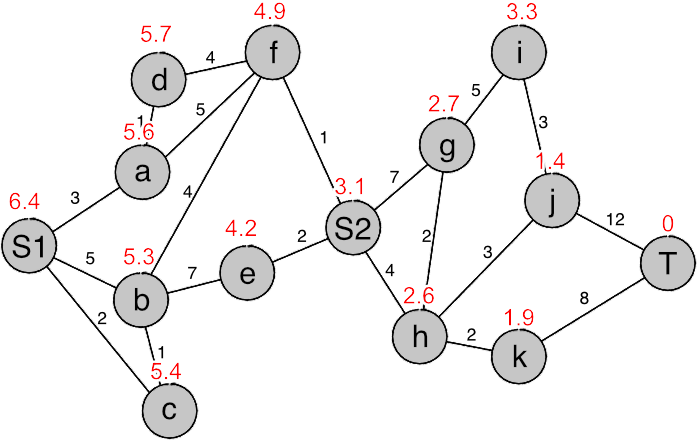
\includegraphics[scale=0.9]{chapters/informed_search/AnfangsproblemHeuristik.png}
	\caption{Beispiel Graph mit Heuristik}
\end{figure}

F\"ur die Suche des k\"urzesten Weges von S1 bzw. S2 nach T ergeben sich die beiden Suchb\"aume B1 (Abbildung6.9) und B2 (Abbildung6.10). Die in blau gekennzeichneten Zahlen geben die Reihenfolge an in der die Pfade begangen werden. Rote Zahlen geben den von der Heuristik gesch\"atzten Wert f\"ur den entsprechenden Knoten an. Die Schwarzen Zahlen geben die tats\"achliche Wegl\"ange vom Startknoten zum betrachteten Knoten an. In lila werden die gesch\"atzten Gesamtkosten eines Knotens angegeben. Als Grau markierte Pfade wurden aufgrund der Extended List ausgeschlossen.

An beiden Suchb\"aumen ist gut zu erkennen, dass viele Abzweigungen aufgrund der Extended List nahezu sofort abgeschnitten werden (gekennzeichnet durch graue Pfade). Am Baum mit Wurzel S2 l\"asst sich der nutzen einer Heuristik nachvollziehen. Die Kosten der Abzweigungen e, f in den linken Teil des Graphen nehmen durch die Heuristik schneller zu und dies sorgt daf\"ur, dass eine Suche dort obsolet (auch durch graue Pfade gekennzeichnet) wird, sobald die gesch\"atzten Kosten gr\"o\ss er als 14 sind (Der k\"urzeste Weg von S2 nach T hat die l\"ange 14). 
Die unterschiedliche Struktur der B\"aume l\"asst sich durch den Startpunkt der Suche erkl\"aren. Aufgrund dessen, dass die Knoten S1 und T auf entgegengesetzten Seiten des Graphen liegen, ergibt sich ein tiefer Baum und da der Knoten S2 den Graphen in zwei Partitionen auftrennt, bildet sich bei der Suche des k\"urzesten Weges von S2 nach T ein breiter Suchbaum. 
\begin{figure}[h!]
	\centering
	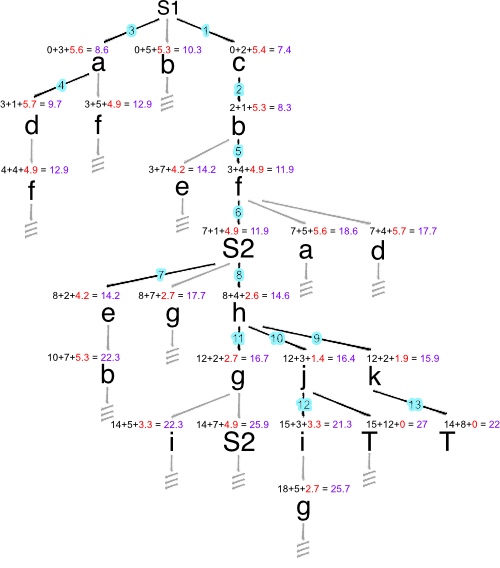
\includegraphics[scale=0.9]{chapters/informed_search/AStarBaum1.png}
	\caption{Such Baum B1 von T nach S1}
	\label{fig:searchtrees1}
\end{figure}

\begin{figure}[h!]
	\centering
	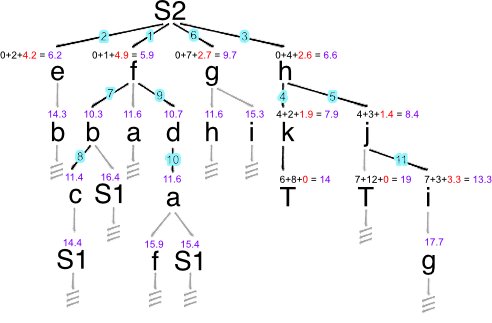
\includegraphics[scale=0.9]{chapters/informed_search/AStarBaum2.png}
	\caption{Such Baum B2 von T nach S2}
	\label{fig:searchtrees2}
\end{figure}
\newpage 